\documentclass[1p]{elsarticle_modified}
%\bibliographystyle{elsarticle-num}

%\usepackage[colorlinks]{hyperref}
%\usepackage{abbrmath_seonhwa} %\Abb, \Ascr, \Acal ,\Abf, \Afrak
\usepackage{amsfonts}
\usepackage{amssymb}
\usepackage{amsmath}
\usepackage{amsthm}
\usepackage{scalefnt}
\usepackage{amsbsy}
\usepackage{kotex}
\usepackage{caption}
\usepackage{subfig}
\usepackage{color}
\usepackage{graphicx}
\usepackage{xcolor} %% white, black, red, green, blue, cyan, magenta, yellow
\usepackage{float}
\usepackage{setspace}
\usepackage{hyperref}

\usepackage{tikz}
\usetikzlibrary{arrows}

\usepackage{multirow}
\usepackage{array} % fixed length table
\usepackage{hhline}

%%%%%%%%%%%%%%%%%%%%%
\makeatletter
\renewcommand*\env@matrix[1][\arraystretch]{%
	\edef\arraystretch{#1}%
	\hskip -\arraycolsep
	\let\@ifnextchar\new@ifnextchar
	\array{*\c@MaxMatrixCols c}}
\makeatother %https://tex.stackexchange.com/questions/14071/how-can-i-increase-the-line-spacing-in-a-matrix
%%%%%%%%%%%%%%%

\usepackage[normalem]{ulem}

\newcommand{\msout}[1]{\ifmmode\text{\sout{\ensuremath{#1}}}\else\sout{#1}\fi}
%SOURCE: \msout is \stkout macro in https://tex.stackexchange.com/questions/20609/strikeout-in-math-mode

\newcommand{\cancel}[1]{
	\ifmmode
	{\color{red}\msout{#1}}
	\else
	{\color{red}\sout{#1}}
	\fi
}

\newcommand{\add}[1]{
	{\color{blue}\uwave{#1}}
}

\newcommand{\replace}[2]{
	\ifmmode
	{\color{red}\msout{#1}}{\color{blue}\uwave{#2}}
	\else
	{\color{red}\sout{#1}}{\color{blue}\uwave{#2}}
	\fi
}

\newcommand{\Sol}{\mathcal{S}} %segment
\newcommand{\D}{D} %diagram
\newcommand{\A}{\mathcal{A}} %arc


%%%%%%%%%%%%%%%%%%%%%%%%%%%%%5 test

\def\sl{\operatorname{\textup{SL}}(2,\Cbb)}
\def\psl{\operatorname{\textup{PSL}}(2,\Cbb)}
\def\quan{\mkern 1mu \triangleright \mkern 1mu}

\theoremstyle{definition}
\newtheorem{thm}{Theorem}[section]
\newtheorem{prop}[thm]{Proposition}
\newtheorem{lem}[thm]{Lemma}
\newtheorem{ques}[thm]{Question}
\newtheorem{cor}[thm]{Corollary}
\newtheorem{defn}[thm]{Definition}
\newtheorem{exam}[thm]{Example}
\newtheorem{rmk}[thm]{Remark}
\newtheorem{alg}[thm]{Algorithm}

\newcommand{\I}{\sqrt{-1}}
\begin{document}

%\begin{frontmatter}
%
%\title{Boundary parabolic representations of knots up to 8 crossings}
%
%%% Group authors per affiliation:
%\author{Yunhi Cho} 
%\address{Department of Mathematics, University of Seoul, Seoul, Korea}
%\ead{yhcho@uos.ac.kr}
%
%
%\author{Seonhwa Kim} %\fnref{s_kim}}
%\address{Center for Geometry and Physics, Institute for Basic Science, Pohang, 37673, Korea}
%\ead{ryeona17@ibs.re.kr}
%
%\author{Hyuk Kim}
%\address{Department of Mathematical Sciences, Seoul National University, Seoul 08826, Korea}
%\ead{hyukkim@snu.ac.kr}
%
%\author{Seokbeom Yoon}
%\address{Department of Mathematical Sciences, Seoul National University, Seoul, 08826,  Korea}
%\ead{sbyoon15@snu.ac.kr}
%
%\begin{abstract}
%We find all boundary parabolic representation of knots up to 8 crossings.
%
%\end{abstract}
%\begin{keyword}
%    \MSC[2010] 57M25 
%\end{keyword}
%
%\end{frontmatter}

%\linenumbers
%\tableofcontents
%
\newcommand\colored[1]{\textcolor{white}{\rule[-0.35ex]{0.8em}{1.4ex}}\kern-0.8em\color{red} #1}%
%\newcommand\colored[1]{\textcolor{white}{ #1}\kern-2.17ex	\textcolor{white}{ #1}\kern-1.81ex	\textcolor{white}{ #1}\kern-2.15ex\color{red}#1	}

{\Large $\underline{12a_{0863}~(K12a_{0863})}$}

\setlength{\tabcolsep}{10pt}
\renewcommand{\arraystretch}{1.6}
\vspace{1cm}\begin{tabular}{m{100pt}>{\centering\arraybackslash}m{274pt}}
\multirow{5}{120pt}{
	\centering
	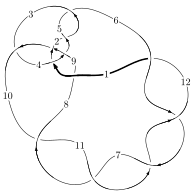
\includegraphics[width=112pt]{../../../GIT/diagram.site/Diagrams/png/1664_12a_0863.png}\\
\ \ \ A knot diagram\footnotemark}&
\allowdisplaybreaks
\textbf{Linearized knot diagam} \\
\cline{2-2}
 &
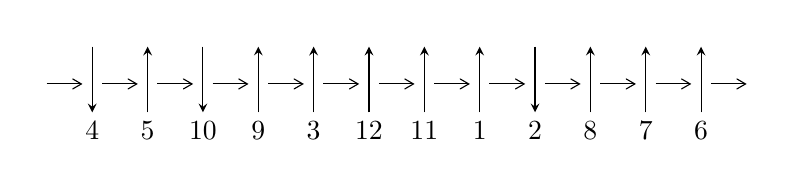
\begin{tikzpicture}[x=20pt, y=17pt]
	% nodes
	\node (C0) at (0, 0) {};
	\node (C1) at (1, 0) {};
	\node (C1U) at (1, +1) {};
	\node (C1D) at (1, -1) {4};

	\node (C2) at (2, 0) {};
	\node (C2U) at (2, +1) {};
	\node (C2D) at (2, -1) {5};

	\node (C3) at (3, 0) {};
	\node (C3U) at (3, +1) {};
	\node (C3D) at (3, -1) {10};

	\node (C4) at (4, 0) {};
	\node (C4U) at (4, +1) {};
	\node (C4D) at (4, -1) {9};

	\node (C5) at (5, 0) {};
	\node (C5U) at (5, +1) {};
	\node (C5D) at (5, -1) {3};

	\node (C6) at (6, 0) {};
	\node (C6U) at (6, +1) {};
	\node (C6D) at (6, -1) {12};

	\node (C7) at (7, 0) {};
	\node (C7U) at (7, +1) {};
	\node (C7D) at (7, -1) {11};

	\node (C8) at (8, 0) {};
	\node (C8U) at (8, +1) {};
	\node (C8D) at (8, -1) {1};

	\node (C9) at (9, 0) {};
	\node (C9U) at (9, +1) {};
	\node (C9D) at (9, -1) {2};

	\node (C10) at (10, 0) {};
	\node (C10U) at (10, +1) {};
	\node (C10D) at (10, -1) {8};

	\node (C11) at (11, 0) {};
	\node (C11U) at (11, +1) {};
	\node (C11D) at (11, -1) {7};

	\node (C12) at (12, 0) {};
	\node (C12U) at (12, +1) {};
	\node (C12D) at (12, -1) {6};
	\node (C13) at (13, 0) {};

	% arrows
	\draw[->,>={angle 60}]
	(C0) edge (C1) (C1) edge (C2) (C2) edge (C3) (C3) edge (C4) (C4) edge (C5) (C5) edge (C6) (C6) edge (C7) (C7) edge (C8) (C8) edge (C9) (C9) edge (C10) (C10) edge (C11) (C11) edge (C12) (C12) edge (C13) ;	\draw[->,>=stealth]
	(C1U) edge (C1D) (C2D) edge (C2U) (C3U) edge (C3D) (C4D) edge (C4U) (C5D) edge (C5U) (C6D) edge (C6U) (C7D) edge (C7U) (C8D) edge (C8U) (C9U) edge (C9D) (C10D) edge (C10U) (C11D) edge (C11U) (C12D) edge (C12U) ;
	\end{tikzpicture} \\
\hhline{~~} \\& 
\textbf{Solving Sequence} \\ \cline{2-2} 
 &
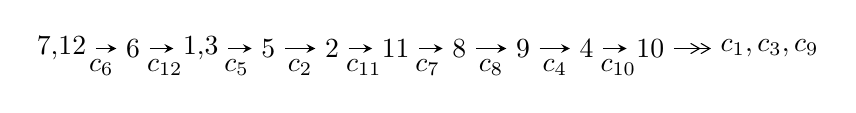
\begin{tikzpicture}[x=23pt, y=7pt]
	% node
	\node (A0) at (-1/8, 0) {7,12};
	\node (A1) at (1, 0) {6};
	\node (A2) at (33/16, 0) {1,3};
	\node (A3) at (25/8, 0) {5};
	\node (A4) at (33/8, 0) {2};
	\node (A5) at (41/8, 0) {11};
	\node (A6) at (49/8, 0) {8};
	\node (A7) at (57/8, 0) {9};
	\node (A8) at (65/8, 0) {4};
	\node (A9) at (73/8, 0) {10};
	\node (C1) at (1/2, -1) {$c_{6}$};
	\node (C2) at (3/2, -1) {$c_{12}$};
	\node (C3) at (21/8, -1) {$c_{5}$};
	\node (C4) at (29/8, -1) {$c_{2}$};
	\node (C5) at (37/8, -1) {$c_{11}$};
	\node (C6) at (45/8, -1) {$c_{7}$};
	\node (C7) at (53/8, -1) {$c_{8}$};
	\node (C8) at (61/8, -1) {$c_{4}$};
	\node (C9) at (69/8, -1) {$c_{10}$};
	\node (A10) at (11, 0) {$c_{1},c_{3},c_{9}$};

	% edge
	\draw[->,>=stealth]	
	(A0) edge (A1) (A1) edge (A2) (A2) edge (A3) (A3) edge (A4) (A4) edge (A5) (A5) edge (A6) (A6) edge (A7) (A7) edge (A8) (A8) edge (A9) ;
	\draw[->>,>={angle 60}]	
	(A9) edge (A10);
\end{tikzpicture} \\ 

\end{tabular} \\

\footnotetext{
The image of knot diagram is generated by the software ``\textbf{Draw programme}" developed by Andrew Bartholomew(\url{http://www.layer8.co.uk/maths/draw/index.htm\#Running-draw}), where we modified some parts for our purpose(\url{https://github.com/CATsTAILs/LinksPainter}).
}\phantom \\ \newline 
\centering \textbf{Ideals for irreducible components\footnotemark of $X_{\text{par}}$} 
 
\begin{align*}
I^u_{1}&=\langle 
-1.21287\times10^{19} u^{64}+1.88559\times10^{21} u^{63}+\cdots+2.29526\times10^{21} b-1.81954\times10^{17},\\
\phantom{I^u_{1}}&\phantom{= \langle  }1.21260\times10^{19} u^{64}-1.88577\times10^{21} u^{63}+\cdots+2.29526\times10^{21} a-4.20780\times10^{21},\;u^{65}- u^{64}+\cdots+3 u+1\rangle \\
\\
\end{align*}
\raggedright * 1 irreducible components of $\dim_{\mathbb{C}}=0$, with total 65 representations.\\
\footnotetext{All coefficients of polynomials are rational numbers. But the coefficients are sometimes approximated in decimal forms when there is not enough margin.}
\newpage
\renewcommand{\arraystretch}{1}
\centering \section*{I. $I^u_{1}= \langle -1.21\times10^{19} u^{64}+1.89\times10^{21} u^{63}+\cdots+2.30\times10^{21} b-1.82\times10^{17},\;1.21\times10^{19} u^{64}-1.89\times10^{21} u^{63}+\cdots+2.30\times10^{21} a-4.21\times10^{21},\;u^{65}- u^{64}+\cdots+3 u+1 \rangle$}
\flushleft \textbf{(i) Arc colorings}\\
\begin{tabular}{m{7pt} m{180pt} m{7pt} m{180pt} }
\flushright $a_{7}=$&$\begin{pmatrix}1\\0\end{pmatrix}$ \\
\flushright $a_{12}=$&$\begin{pmatrix}0\\u\end{pmatrix}$ \\
\flushright $a_{6}=$&$\begin{pmatrix}1\\u^2\end{pmatrix}$ \\
\flushright $a_{1}=$&$\begin{pmatrix}u\\u^3+u\end{pmatrix}$ \\
\flushright $a_{3}=$&$\begin{pmatrix}-0.00528304 u^{64}+0.821593 u^{63}+\cdots-3.85538 u+1.83325\\0.00528425 u^{64}-0.821515 u^{63}+\cdots-3.16643 u+0.0000792739\end{pmatrix}$ \\
\flushright $a_{5}=$&$\begin{pmatrix}0.00446144 u^{64}+0.730022 u^{63}+\cdots-5.30127 u+2.48337\\-0.00446223 u^{64}-0.730061 u^{63}+\cdots-3.31679 u-0.0000393275\end{pmatrix}$ \\
\flushright $a_{2}=$&$\begin{pmatrix}0.00281825 u^{64}+0.833252 u^{63}+\cdots+4.38543 u+0.116626\\-0.00281820 u^{64}-0.833212 u^{63}+\cdots+0.716788 u+0.0000405652\end{pmatrix}$ \\
\flushright $a_{11}=$&$\begin{pmatrix}- u\\u\end{pmatrix}$ \\
\flushright $a_{8}=$&$\begin{pmatrix}u^2+1\\- u^2\end{pmatrix}$ \\
\flushright $a_{9}=$&$\begin{pmatrix}- u^6-3 u^4+1\\- u^8-4 u^6-4 u^4-2 u^2\end{pmatrix}$ \\
\flushright $a_{4}=$&$\begin{pmatrix}0.000622185 u^{64}+0.0750748 u^{63}+\cdots-3.85513 u+1.83334\\-0.000622272 u^{64}-0.0750774 u^{63}+\cdots-3.16667 u-2.69978\times10^{-6}\end{pmatrix}$ \\
\flushright $a_{10}=$&$\begin{pmatrix}- u^3-2 u\\u^3+u\end{pmatrix}$\\&\end{tabular}
\flushleft \textbf{(ii) Obstruction class $= -1$}\\~\\
\flushleft \textbf{(iii) Cusp Shapes $= -\frac{7390754013604632808088}{2295261755894092887829} u^{64}+\frac{5553779548253673895596}{2295261755894092887829} u^{63}+\cdots+\frac{14535116494160491630104}{2295261755894092887829} u+\frac{12347743172761319269322}{2295261755894092887829}$}\\~\\
\newpage\renewcommand{\arraystretch}{1}
\flushleft \textbf{(iv) u-Polynomials at the component}\newline \\
\begin{tabular}{m{50pt}|m{274pt}}
Crossings & \hspace{64pt}u-Polynomials at each crossing \\
\hline $$\begin{aligned}c_{1}\end{aligned}$$&$\begin{aligned}
&u^{65}-11 u^{64}+\cdots- u+1
\end{aligned}$\\
\hline $$\begin{aligned}c_{2},c_{5}\end{aligned}$$&$\begin{aligned}
&u^{65}+u^{64}+\cdots+11 u-1
\end{aligned}$\\
\hline $$\begin{aligned}c_{3}\end{aligned}$$&$\begin{aligned}
&u^{65}+u^{64}+\cdots-587 u+953
\end{aligned}$\\
\hline $$\begin{aligned}c_{4}\end{aligned}$$&$\begin{aligned}
&u^{65}+3 u^{64}+\cdots+963 u+251
\end{aligned}$\\
\hline $$\begin{aligned}c_{6},c_{7},c_{10}\\c_{11},c_{12}\end{aligned}$$&$\begin{aligned}
&u^{65}+u^{64}+\cdots+3 u-1
\end{aligned}$\\
\hline $$\begin{aligned}c_{8}\end{aligned}$$&$\begin{aligned}
&u^{65}+u^{64}+\cdots-107 u-1
\end{aligned}$\\
\hline $$\begin{aligned}c_{9}\end{aligned}$$&$\begin{aligned}
&u^{65}-3 u^{64}+\cdots- u+1
\end{aligned}$\\
\hline
\end{tabular}\\~\\
\newpage\renewcommand{\arraystretch}{1}
\flushleft \textbf{(v) Riley Polynomials at the component}\newline \\
\begin{tabular}{m{50pt}|m{274pt}}
Crossings & \hspace{64pt}Riley Polynomials at each crossing \\
\hline $$\begin{aligned}c_{1}\end{aligned}$$&$\begin{aligned}
&y^{65}+3 y^{64}+\cdots-11 y-1
\end{aligned}$\\
\hline $$\begin{aligned}c_{2},c_{5}\end{aligned}$$&$\begin{aligned}
&y^{65}-45 y^{64}+\cdots-11 y-1
\end{aligned}$\\
\hline $$\begin{aligned}c_{3}\end{aligned}$$&$\begin{aligned}
&y^{65}-45 y^{64}+\cdots-18627755 y-908209
\end{aligned}$\\
\hline $$\begin{aligned}c_{4}\end{aligned}$$&$\begin{aligned}
&y^{65}-73 y^{64}+\cdots+2575937 y-63001
\end{aligned}$\\
\hline $$\begin{aligned}c_{6},c_{7},c_{10}\\c_{11},c_{12}\end{aligned}$$&$\begin{aligned}
&y^{65}+83 y^{64}+\cdots-3 y-1
\end{aligned}$\\
\hline $$\begin{aligned}c_{8}\end{aligned}$$&$\begin{aligned}
&y^{65}-21 y^{64}+\cdots+6349 y-1
\end{aligned}$\\
\hline $$\begin{aligned}c_{9}\end{aligned}$$&$\begin{aligned}
&y^{65}+11 y^{64}+\cdots-3 y-1
\end{aligned}$\\
\hline
\end{tabular}\\~\\
\newpage\flushleft \textbf{(vi) Complex Volumes and Cusp Shapes}
$$\begin{array}{c|c|c}  
\text{Solutions to }I^u_{1}& \I (\text{vol} + \sqrt{-1}CS) & \text{Cusp shape}\\
 \hline 
\begin{aligned}
u &= \phantom{-}0.324128 + 0.936130 I \\
a &= -1.09302 + 1.30299 I \\
b &= \phantom{-}0.082181 - 0.503434 I\end{aligned}
 & -2.40034 + 7.24090 I & \phantom{-0.000000 } 0 \\ \hline\begin{aligned}
u &= \phantom{-}0.324128 - 0.936130 I \\
a &= -1.09302 - 1.30299 I \\
b &= \phantom{-}0.082181 + 0.503434 I\end{aligned}
 & -2.40034 - 7.24090 I & \phantom{-0.000000 } 0 \\ \hline\begin{aligned}
u &= \phantom{-}0.058124 + 1.021150 I \\
a &= \phantom{-}0.39135 - 1.54603 I \\
b &= -0.539037 + 0.901278 I\end{aligned}
 & -5.27537 - 0.99487 I & \phantom{-0.000000 } 0 \\ \hline\begin{aligned}
u &= \phantom{-}0.058124 - 1.021150 I \\
a &= \phantom{-}0.39135 + 1.54603 I \\
b &= -0.539037 - 0.901278 I\end{aligned}
 & -5.27537 + 0.99487 I & \phantom{-0.000000 } 0 \\ \hline\begin{aligned}
u &= -0.269057 + 0.937054 I \\
a &= \phantom{-}0.284515 - 0.610952 I \\
b &= -0.532484 + 0.070320 I\end{aligned}
 & -2.06253 - 2.90913 I & \phantom{-0.000000 } 0 \\ \hline\begin{aligned}
u &= -0.269057 - 0.937054 I \\
a &= \phantom{-}0.284515 + 0.610952 I \\
b &= -0.532484 - 0.070320 I\end{aligned}
 & -2.06253 + 2.90913 I & \phantom{-0.000000 } 0 \\ \hline\begin{aligned}
u &= \phantom{-}0.385420 + 0.961736 I \\
a &= \phantom{-}0.23634 - 2.24647 I \\
b &= \phantom{-}0.104185 + 1.382700 I\end{aligned}
 & \phantom{-}2.02839 + 13.16090 I & \phantom{-0.000000 } 0 \\ \hline\begin{aligned}
u &= \phantom{-}0.385420 - 0.961736 I \\
a &= \phantom{-}0.23634 + 2.24647 I \\
b &= \phantom{-}0.104185 - 1.382700 I\end{aligned}
 & \phantom{-}2.02839 - 13.16090 I & \phantom{-0.000000 } 0 \\ \hline\begin{aligned}
u &= -0.429847 + 0.964672 I \\
a &= \phantom{-}0.078850 + 1.312400 I \\
b &= -0.087710 - 0.887262 I\end{aligned}
 & \phantom{-}0.89662 - 4.74808 I & \phantom{-0.000000 } 0 \\ \hline\begin{aligned}
u &= -0.429847 - 0.964672 I \\
a &= \phantom{-}0.078850 - 1.312400 I \\
b &= -0.087710 + 0.887262 I\end{aligned}
 & \phantom{-}0.89662 + 4.74808 I & \phantom{-0.000000 } 0\\
 \hline 
 \end{array}$$\newpage$$\begin{array}{c|c|c}  
\text{Solutions to }I^u_{1}& \I (\text{vol} + \sqrt{-1}CS) & \text{Cusp shape}\\
 \hline 
\begin{aligned}
u &= \phantom{-}0.314439 + 0.872956 I \\
a &= -0.31327 + 2.44697 I \\
b &= \phantom{-}0.259549 - 1.127420 I\end{aligned}
 & \phantom{-}2.14552 + 4.73651 I & \phantom{-0.000000 } 0 \\ \hline\begin{aligned}
u &= \phantom{-}0.314439 - 0.872956 I \\
a &= -0.31327 - 2.44697 I \\
b &= \phantom{-}0.259549 + 1.127420 I\end{aligned}
 & \phantom{-}2.14552 - 4.73651 I & \phantom{-0.000000 } 0 \\ \hline\begin{aligned}
u &= -0.261979 + 0.871741 I \\
a &= -2.35233 - 2.92298 I \\
b &= \phantom{-}1.35421 + 3.02563 I\end{aligned}
 & \phantom{-}0.12711 - 2.45591 I & \phantom{-0.000000 } 0 \\ \hline\begin{aligned}
u &= -0.261979 - 0.871741 I \\
a &= -2.35233 + 2.92298 I \\
b &= \phantom{-}1.35421 - 3.02563 I\end{aligned}
 & \phantom{-}0.12711 + 2.45591 I & \phantom{-0.000000 } 0 \\ \hline\begin{aligned}
u &= \phantom{-}0.289053 + 0.805920 I \\
a &= \phantom{-}0.560101 + 0.910910 I \\
b &= \phantom{-}0.769764 - 0.657178 I\end{aligned}
 & \phantom{-}2.61125 + 0.92001 I & \phantom{-}10.35838 - 1.61741 I \\ \hline\begin{aligned}
u &= \phantom{-}0.289053 - 0.805920 I \\
a &= \phantom{-}0.560101 - 0.910910 I \\
b &= \phantom{-}0.769764 + 0.657178 I\end{aligned}
 & \phantom{-}2.61125 - 0.92001 I & \phantom{-}10.35838 + 1.61741 I \\ \hline\begin{aligned}
u &= -0.162835 + 0.838324 I \\
a &= \phantom{-}1.67399 + 0.87780 I \\
b &= -0.280248 - 1.013690 I\end{aligned}
 & -0.87255 - 1.60805 I & \phantom{-}6.00000 + 5.45317 I \\ \hline\begin{aligned}
u &= -0.162835 - 0.838324 I \\
a &= \phantom{-}1.67399 - 0.87780 I \\
b &= -0.280248 + 1.013690 I\end{aligned}
 & -0.87255 + 1.60805 I & \phantom{-}6.00000 - 5.45317 I \\ \hline\begin{aligned}
u &= -0.092628 + 1.180290 I \\
a &= -0.840978 + 0.802329 I \\
b &= \phantom{-}0.236084 - 0.580343 I\end{aligned}
 & -2.83299 - 5.08772 I & \phantom{-0.000000 } 0 \\ \hline\begin{aligned}
u &= -0.092628 - 1.180290 I \\
a &= -0.840978 - 0.802329 I \\
b &= \phantom{-}0.236084 + 0.580343 I\end{aligned}
 & -2.83299 + 5.08772 I & \phantom{-0.000000 } 0\\
 \hline 
 \end{array}$$\newpage$$\begin{array}{c|c|c}  
\text{Solutions to }I^u_{1}& \I (\text{vol} + \sqrt{-1}CS) & \text{Cusp shape}\\
 \hline 
\begin{aligned}
u &= -0.532472 + 0.581936 I \\
a &= \phantom{-}0.359653 + 0.752618 I \\
b &= -0.697410 - 0.164439 I\end{aligned}
 & \phantom{-}3.09795 - 3.00575 I & \phantom{-}14.1045 + 10.0032 I \\ \hline\begin{aligned}
u &= -0.532472 - 0.581936 I \\
a &= \phantom{-}0.359653 - 0.752618 I \\
b &= -0.697410 + 0.164439 I\end{aligned}
 & \phantom{-}3.09795 + 3.00575 I & \phantom{-}14.1045 - 10.0032 I \\ \hline\begin{aligned}
u &= \phantom{-}0.451917 + 0.639368 I \\
a &= -0.029660 - 0.522836 I \\
b &= -1.028710 + 0.520293 I\end{aligned}
 & \phantom{-}3.91640 - 6.17027 I & \phantom{-}7.07971 + 2.30194 I \\ \hline\begin{aligned}
u &= \phantom{-}0.451917 - 0.639368 I \\
a &= -0.029660 + 0.522836 I \\
b &= -1.028710 - 0.520293 I\end{aligned}
 & \phantom{-}3.91640 + 6.17027 I & \phantom{-}7.07971 - 2.30194 I \\ \hline\begin{aligned}
u &= -0.680129 + 0.170323 I \\
a &= \phantom{-}1.001600 + 0.629885 I \\
b &= -0.553761 + 0.076940 I\end{aligned}
 & \phantom{-}4.35899 - 1.00540 I & \phantom{-}20.7008 + 5.0169 I \\ \hline\begin{aligned}
u &= -0.680129 - 0.170323 I \\
a &= \phantom{-}1.001600 - 0.629885 I \\
b &= -0.553761 - 0.076940 I\end{aligned}
 & \phantom{-}4.35899 + 1.00540 I & \phantom{-}20.7008 - 5.0169 I \\ \hline\begin{aligned}
u &= \phantom{-}0.619172 + 0.144302 I \\
a &= \phantom{-}1.59691 - 0.92448 I \\
b &= -0.623408 - 0.537423 I\end{aligned}
 & \phantom{-}5.42013 + 9.76545 I & \phantom{-}9.79000 - 7.37220 I \\ \hline\begin{aligned}
u &= \phantom{-}0.619172 - 0.144302 I \\
a &= \phantom{-}1.59691 + 0.92448 I \\
b &= -0.623408 + 0.537423 I\end{aligned}
 & \phantom{-}5.42013 - 9.76545 I & \phantom{-}9.79000 + 7.37220 I \\ \hline\begin{aligned}
u &= \phantom{-}0.205923 + 0.598857 I \\
a &= \phantom{-}1.29669 - 0.57305 I \\
b &= -0.059987 - 0.280461 I\end{aligned}
 & -0.66580 - 1.57263 I & \phantom{-}3.10575 + 2.35415 I \\ \hline\begin{aligned}
u &= \phantom{-}0.205923 - 0.598857 I \\
a &= \phantom{-}1.29669 + 0.57305 I \\
b &= -0.059987 + 0.280461 I\end{aligned}
 & -0.66580 + 1.57263 I & \phantom{-}3.10575 - 2.35415 I\\
 \hline 
 \end{array}$$\newpage$$\begin{array}{c|c|c}  
\text{Solutions to }I^u_{1}& \I (\text{vol} + \sqrt{-1}CS) & \text{Cusp shape}\\
 \hline 
\begin{aligned}
u &= -0.010335 + 0.617504 I \\
a &= \phantom{-}1.307680 - 0.534985 I \\
b &= -0.197340 - 0.348140 I\end{aligned}
 & -0.65799 - 1.53035 I & \phantom{-}2.49577 + 4.53431 I \\ \hline\begin{aligned}
u &= -0.010335 - 0.617504 I \\
a &= \phantom{-}1.307680 + 0.534985 I \\
b &= -0.197340 + 0.348140 I\end{aligned}
 & -0.65799 + 1.53035 I & \phantom{-}2.49577 - 4.53431 I \\ \hline\begin{aligned}
u &= \phantom{-}0.528313 + 0.122256 I \\
a &= -0.528984 - 0.299527 I \\
b &= \phantom{-}0.005243 + 0.913496 I\end{aligned}
 & \phantom{-}0.83726 + 4.33484 I & \phantom{-}8.01107 - 7.64767 I \\ \hline\begin{aligned}
u &= \phantom{-}0.528313 - 0.122256 I \\
a &= -0.528984 + 0.299527 I \\
b &= \phantom{-}0.005243 - 0.913496 I\end{aligned}
 & \phantom{-}0.83726 - 4.33484 I & \phantom{-}8.01107 + 7.64767 I \\ \hline\begin{aligned}
u &= \phantom{-}0.524320 + 0.036054 I \\
a &= -2.00699 + 0.30540 I \\
b &= \phantom{-}0.874865 + 0.548909 I\end{aligned}
 & \phantom{-}4.90067 + 1.87571 I & \phantom{-}15.7861 - 4.1218 I \\ \hline\begin{aligned}
u &= \phantom{-}0.524320 - 0.036054 I \\
a &= -2.00699 - 0.30540 I \\
b &= \phantom{-}0.874865 - 0.548909 I\end{aligned}
 & \phantom{-}4.90067 - 1.87571 I & \phantom{-}15.7861 + 4.1218 I \\ \hline\begin{aligned}
u &= -0.458267\phantom{ +0.000000I} \\
a &= -6.03074\phantom{ +0.000000I} \\
b &= -0.211824\phantom{ +0.000000I}\end{aligned}
 & \phantom{-}2.77275\phantom{ +0.000000I} & -28.7580\phantom{ +0.000000I} \\ \hline\begin{aligned}
u &= -0.445497 + 0.094527 I \\
a &= \phantom{-}0.637012 - 0.423531 I \\
b &= \phantom{-}0.226599 - 0.250291 I\end{aligned}
 & \phantom{-}1.107960 - 0.463162 I & \phantom{-}9.21159 + 1.20629 I \\ \hline\begin{aligned}
u &= -0.445497 - 0.094527 I \\
a &= \phantom{-}0.637012 + 0.423531 I \\
b &= \phantom{-}0.226599 + 0.250291 I\end{aligned}
 & \phantom{-}1.107960 + 0.463162 I & \phantom{-}9.21159 - 1.20629 I \\ \hline\begin{aligned}
u &= \phantom{-}0.02751 + 1.56537 I \\
a &= -0.432111 + 0.242266 I \\
b &= -0.285023 - 0.338181 I\end{aligned}
 & -3.27465 - 4.58250 I & \phantom{-0.000000 } 0\\
 \hline 
 \end{array}$$\newpage$$\begin{array}{c|c|c}  
\text{Solutions to }I^u_{1}& \I (\text{vol} + \sqrt{-1}CS) & \text{Cusp shape}\\
 \hline 
\begin{aligned}
u &= \phantom{-}0.02751 - 1.56537 I \\
a &= -0.432111 - 0.242266 I \\
b &= -0.285023 + 0.338181 I\end{aligned}
 & -3.27465 + 4.58250 I & \phantom{-0.000000 } 0 \\ \hline\begin{aligned}
u &= \phantom{-}0.03404 + 1.66686 I \\
a &= \phantom{-}1.11783 - 1.17422 I \\
b &= -2.37959 + 2.42684 I\end{aligned}
 & -9.12781 - 0.99471 I & \phantom{-0.000000 } 0 \\ \hline\begin{aligned}
u &= \phantom{-}0.03404 - 1.66686 I \\
a &= \phantom{-}1.11783 + 1.17422 I \\
b &= -2.37959 - 2.42684 I\end{aligned}
 & -9.12781 + 0.99471 I & \phantom{-0.000000 } 0 \\ \hline\begin{aligned}
u &= \phantom{-}0.06301 + 1.66986 I \\
a &= \phantom{-}1.005040 + 0.262704 I \\
b &= -1.22784 - 0.87146 I\end{aligned}
 & -6.11147 + 2.17232 I & \phantom{-0.000000 } 0 \\ \hline\begin{aligned}
u &= \phantom{-}0.06301 - 1.66986 I \\
a &= \phantom{-}1.005040 - 0.262704 I \\
b &= -1.22784 + 0.87146 I\end{aligned}
 & -6.11147 - 2.17232 I & \phantom{-0.000000 } 0 \\ \hline\begin{aligned}
u &= \phantom{-}0.07662 + 1.68231 I \\
a &= \phantom{-}0.45152 + 2.14712 I \\
b &= -0.42780 - 5.18456 I\end{aligned}
 & -6.84024 + 6.21304 I & \phantom{-0.000000 } 0 \\ \hline\begin{aligned}
u &= \phantom{-}0.07662 - 1.68231 I \\
a &= \phantom{-}0.45152 - 2.14712 I \\
b &= -0.42780 + 5.18456 I\end{aligned}
 & -6.84024 - 6.21304 I & \phantom{-0.000000 } 0 \\ \hline\begin{aligned}
u &= -0.04521 + 1.68391 I \\
a &= \phantom{-}1.25462 + 1.36266 I \\
b &= -2.68362 - 3.82166 I\end{aligned}
 & -9.85939 - 2.43463 I & \phantom{-0.000000 } 0 \\ \hline\begin{aligned}
u &= -0.04521 - 1.68391 I \\
a &= \phantom{-}1.25462 - 1.36266 I \\
b &= -2.68362 + 3.82166 I\end{aligned}
 & -9.85939 + 2.43463 I & \phantom{-0.000000 } 0 \\ \hline\begin{aligned}
u &= -0.06445 + 1.68600 I \\
a &= -1.21200 - 2.26617 I \\
b &= \phantom{-}4.03468 + 6.58326 I\end{aligned}
 & -8.91650 - 3.69377 I & \phantom{-0.000000 } 0\\
 \hline 
 \end{array}$$\newpage$$\begin{array}{c|c|c}  
\text{Solutions to }I^u_{1}& \I (\text{vol} + \sqrt{-1}CS) & \text{Cusp shape}\\
 \hline 
\begin{aligned}
u &= -0.06445 - 1.68600 I \\
a &= -1.21200 + 2.26617 I \\
b &= \phantom{-}4.03468 - 6.58326 I\end{aligned}
 & -8.91650 + 3.69377 I & \phantom{-0.000000 } 0 \\ \hline\begin{aligned}
u &= \phantom{-}0.08391 + 1.69898 I \\
a &= -0.73541 + 1.68409 I \\
b &= \phantom{-}1.62720 - 3.82199 I\end{aligned}
 & -11.6884 + 8.8421 I & \phantom{-0.000000 } 0 \\ \hline\begin{aligned}
u &= \phantom{-}0.08391 - 1.69898 I \\
a &= -0.73541 - 1.68409 I \\
b &= \phantom{-}1.62720 + 3.82199 I\end{aligned}
 & -11.6884 - 8.8421 I & \phantom{-0.000000 } 0 \\ \hline\begin{aligned}
u &= -0.07063 + 1.70293 I \\
a &= \phantom{-}0.154544 - 0.773326 I \\
b &= -0.67957 + 1.80754 I\end{aligned}
 & -11.41960 - 4.25212 I & \phantom{-0.000000 } 0 \\ \hline\begin{aligned}
u &= -0.07063 - 1.70293 I \\
a &= \phantom{-}0.154544 + 0.773326 I \\
b &= -0.67957 - 1.80754 I\end{aligned}
 & -11.41960 + 4.25212 I & \phantom{-0.000000 } 0 \\ \hline\begin{aligned}
u &= -0.11448 + 1.70115 I \\
a &= -0.284828 + 1.185120 I \\
b &= \phantom{-}0.15081 - 3.05011 I\end{aligned}
 & -8.41150 - 6.90652 I & \phantom{-0.000000 } 0 \\ \hline\begin{aligned}
u &= -0.11448 - 1.70115 I \\
a &= -0.284828 - 1.185120 I \\
b &= \phantom{-}0.15081 + 3.05011 I\end{aligned}
 & -8.41150 + 6.90652 I & \phantom{-0.000000 } 0 \\ \hline\begin{aligned}
u &= \phantom{-}0.10323 + 1.70470 I \\
a &= -0.40089 - 2.00987 I \\
b &= \phantom{-}0.48020 + 5.10501 I\end{aligned}
 & -7.3366 + 15.1066 I & \phantom{-0.000000 } 0 \\ \hline\begin{aligned}
u &= \phantom{-}0.10323 - 1.70470 I \\
a &= -0.40089 + 2.00987 I \\
b &= \phantom{-}0.48020 - 5.10501 I\end{aligned}
 & -7.3366 - 15.1066 I & \phantom{-0.000000 } 0 \\ \hline\begin{aligned}
u &= \phantom{-}0.01436 + 1.71792 I \\
a &= \phantom{-}0.02953 - 1.66944 I \\
b &= -0.45613 + 4.08328 I\end{aligned}
 & -15.0478 - 0.7036 I & \phantom{-0.000000 } 0\\
 \hline 
 \end{array}$$\newpage$$\begin{array}{c|c|c}  
\text{Solutions to }I^u_{1}& \I (\text{vol} + \sqrt{-1}CS) & \text{Cusp shape}\\
 \hline 
\begin{aligned}
u &= \phantom{-}0.01436 - 1.71792 I \\
a &= \phantom{-}0.02953 + 1.66944 I \\
b &= -0.45613 - 4.08328 I\end{aligned}
 & -15.0478 + 0.7036 I & \phantom{-0.000000 } 0 \\ \hline\begin{aligned}
u &= -0.01921 + 1.74361 I \\
a &= -1.01827 + 1.00574 I \\
b &= \phantom{-}2.14452 - 2.51876 I\end{aligned}
 & -13.2560 - 5.5225 I & \phantom{-0.000000 } 0 \\ \hline\begin{aligned}
u &= -0.01921 - 1.74361 I \\
a &= -1.01827 - 1.00574 I \\
b &= \phantom{-}2.14452 + 2.51876 I\end{aligned}
 & -13.2560 + 5.5225 I & \phantom{-0.000000 } 0 \\ \hline\begin{aligned}
u &= -0.175614 + 0.182608 I \\
a &= \phantom{-}2.82636 - 0.76498 I \\
b &= \phantom{-}0.995509 - 0.313938 I\end{aligned}
 & \phantom{-}1.92909 - 0.63355 I & \phantom{-}4.68520 - 2.34882 I \\ \hline\begin{aligned}
u &= -0.175614 - 0.182608 I \\
a &= \phantom{-}2.82636 + 0.76498 I \\
b &= \phantom{-}0.995509 + 0.313938 I\end{aligned}
 & \phantom{-}1.92909 + 0.63355 I & \phantom{-}4.68520 + 2.34882 I\\
 \hline 
 \end{array}$$\newpage
\newpage\renewcommand{\arraystretch}{1}
\centering \section*{ II. u-Polynomials}
\begin{tabular}{m{50pt}|m{274pt}}
Crossings & \hspace{64pt}u-Polynomials at each crossing \\
\hline $$\begin{aligned}c_{1}\end{aligned}$$&$\begin{aligned}
&u^{65}-11 u^{64}+\cdots- u+1
\end{aligned}$\\
\hline $$\begin{aligned}c_{2},c_{5}\end{aligned}$$&$\begin{aligned}
&u^{65}+u^{64}+\cdots+11 u-1
\end{aligned}$\\
\hline $$\begin{aligned}c_{3}\end{aligned}$$&$\begin{aligned}
&u^{65}+u^{64}+\cdots-587 u+953
\end{aligned}$\\
\hline $$\begin{aligned}c_{4}\end{aligned}$$&$\begin{aligned}
&u^{65}+3 u^{64}+\cdots+963 u+251
\end{aligned}$\\
\hline $$\begin{aligned}c_{6},c_{7},c_{10}\\c_{11},c_{12}\end{aligned}$$&$\begin{aligned}
&u^{65}+u^{64}+\cdots+3 u-1
\end{aligned}$\\
\hline $$\begin{aligned}c_{8}\end{aligned}$$&$\begin{aligned}
&u^{65}+u^{64}+\cdots-107 u-1
\end{aligned}$\\
\hline $$\begin{aligned}c_{9}\end{aligned}$$&$\begin{aligned}
&u^{65}-3 u^{64}+\cdots- u+1
\end{aligned}$\\
\hline
\end{tabular}\newpage\renewcommand{\arraystretch}{1}
\centering \section*{ III. Riley Polynomials}
\begin{tabular}{m{50pt}|m{274pt}}
Crossings & \hspace{64pt}Riley Polynomials at each crossing \\
\hline $$\begin{aligned}c_{1}\end{aligned}$$&$\begin{aligned}
&y^{65}+3 y^{64}+\cdots-11 y-1
\end{aligned}$\\
\hline $$\begin{aligned}c_{2},c_{5}\end{aligned}$$&$\begin{aligned}
&y^{65}-45 y^{64}+\cdots-11 y-1
\end{aligned}$\\
\hline $$\begin{aligned}c_{3}\end{aligned}$$&$\begin{aligned}
&y^{65}-45 y^{64}+\cdots-18627755 y-908209
\end{aligned}$\\
\hline $$\begin{aligned}c_{4}\end{aligned}$$&$\begin{aligned}
&y^{65}-73 y^{64}+\cdots+2575937 y-63001
\end{aligned}$\\
\hline $$\begin{aligned}c_{6},c_{7},c_{10}\\c_{11},c_{12}\end{aligned}$$&$\begin{aligned}
&y^{65}+83 y^{64}+\cdots-3 y-1
\end{aligned}$\\
\hline $$\begin{aligned}c_{8}\end{aligned}$$&$\begin{aligned}
&y^{65}-21 y^{64}+\cdots+6349 y-1
\end{aligned}$\\
\hline $$\begin{aligned}c_{9}\end{aligned}$$&$\begin{aligned}
&y^{65}+11 y^{64}+\cdots-3 y-1
\end{aligned}$\\
\hline
\end{tabular}
\vskip 2pc
\end{document}